\documentclass[a4paper, 12pt, parskip=half]{scrbook}

% Einfaches Copy and Paste ermöglichen
\usepackage{cmap}

% deutsche Silbentrennung
\usepackage[ngerman]{babel}

% deutsche Umlaute
\usepackage[utf8]{inputenc}
\usepackage[T1]{fontenc}

\usepackage{csquotes}

% Keine extra Leerzeichen nach einem Punkt
\frenchspacing

% Schriftart
\usepackage{times}

% Stichwortverzeichnis
\usepackage{imakeidx}
\makeindex

% Paket für Änderungen an Kopf- und Fußzeile
\usepackage{scrlayer-scrpage}
% Bisherige Einstellungen für Kopf- und Fußzeilen löschen:
\clearpairofpagestyles
% Einstellungen für die Fußzeile, die Kopfzeile wird nicht verwendet
	% Einstellungen nur für die rechten Seiten
	% Layout: |  Seite
\rofoot[\textbf{$\mid$~~\pagemark}]{\textbf{$\mid$~~\pagemark}}
	% Einstellungen nur für die linken Seiten
	% Layout: Seite  |
\lefoot[\textbf{\pagemark~~$\mid$}]{\textbf{\pagemark~~$\mid$}}

% Paket für code Beispiele
\usepackage{listings}

% Paket für Komma getrennte Fußnoten
\usepackage[multiple]{footmisc}

% Paket für Verlinkungen
\PassOptionsToPackage{hyphens}{url}\usepackage[breaklinks]{hyperref}

\renewcommand{\UrlBreaks}{\do\/\do\-\do\_\do\&\do\?}	% allows URL breaking on /, -, _ and &

% Eigene Commands
\newcommand{\thesisTitle}{Vorläufiges Thema}
\newcommand{\thesisSubject}{Vorläufiges Subject}
\newcommand{\thesisAuthor}{Robert Hartings}
\newcommand{\Matrikelnummer}{1164453}


% Literaturverzeichnis einrichten
\usepackage[style=alphabetic, citestyle=alphabetic]{biblatex}
\addbibresource{thesis.bib}

\hypersetup{
	unicode = true, % allows to use characters of non-Latin based languages in Acrobat’s bookmarks 
	pdftitle = {\thesisTitle}, % define the title that gets displayed in the "Document Info" window of Acrobat 
	pdfauthor = {\thesisAuthor},
	pdfsubject = {\thesisSubject},
	pdfkeywords = {ITS2, hack-me-if-you-can},
	colorlinks = true,
	citecolor = black,
	filecolor = black,
	linkcolor = black,
	urlcolor = black,
	linktoc = all,
}

\title{\thesisTitle}
\author{\thesisAuthor}
\date{\today{}}

\begin{document}
	% Vorspann einleiten:
	\frontmatter
	
	\begin{titlepage}
	
\begin{center}
		\textbf{\Large Entwurf und Realisierung eines}\\
		\textbf{\Large Capture the Flag Core Systems}\\[3cm]
		\textbf{Bachelorarbeit}\\
		zur Erlangung des Grades {\em Bachelor of Science}\\[1.5cm]
		
		an der\\
		Hochschule Niederrhein\\
		Fachbereich Elektrotechnik und Informatik\\
		Studiengang {\em Informatik}\\[3cm]
		
		vorgelegt von\\
		\thesisAuthor\\
		Matrikelnummer: \Matrikelnummer\\[3cm]
		Datum: 4. August 2020\\[3cm]
		
		Prüfer:~Prof.~Dr.~Jürgen Quade\\
		Zweitprüfer:~Prof.~Dr.~Peter~Davids
	\end{center}
\end{titlepage}
	\cleardoublepage
	\pagestyle{scrheadings}
	%-------------------------------------
\section*{Eidesstattliche Erklärung}
%-------------------------------------

\begin{tabbing}
	Matrikelnummer: \= \kill
	Name: \> \thesisAuthor\\
	Matrikelnr.: \> \Matrikelnummer\\
	Titel: \> \thesisTitle\\
	Englischer Titel: \> \thesisTitleEnglish\\
\end{tabbing}

Ich versichere durch meine Unterschrift, dass die vorliegende Arbeit ausschließlich von mir verfasst wurde.
Es wurden keine anderen als die von mir angegebenen Quellen und Hilfsmittel benutzt.

Die Arbeit besteht aus \underline{\hspace{3em}} Seiten.

\vspace{6ex}
\begin{tabbing}
\underline{\hspace{14em}} \hspace{3em}\= \underline{\hspace{14em}} \\
Ort, Datum \> \thesisAuthor
\end{tabbing}
	\tableofcontents	

	
	% Hauptteil einleiten:
	\mainmatter
	
	% Einstellungen für die Fußzeile aktualisieren
		% Einstellungen nur für die rechten Seiten
		% Layout: Abschnitt  |  Seite
	\rofoot[\textbf{\headmark~~$\mid$~~\pagemark}]{\textbf{\headmark~~$\mid$~~\pagemark}}
		% Einstellungen nur für die linken Seiten
		% Layout: Seite  |  Kapitel
	\lefoot[\textbf{\pagemark~~$\mid$~~Kapitel~\headmark}]{\textbf{\pagemark~~$\mid$~~Kapitel~\headmark}}
	
	\chapter{Einleitung}
	\label{chap:Einleitung}
	\label{chap_text:Einleitung}
Das Thema IT Sicherheit ist besonders in den letzten Jahren relevant geworden. Viele Firmen suchen Fachkundige \cite{it-daily.netITSecurityExpertenWerdenHanderingend2019}, die die bestehenden und neu designten Systeme und Programme auf Sicherheitslücken prüfen und Lösungsvorschläge zu deren Behebung präsentieren. Auch werden Experten gesucht, die die im Unternehmen bestehenden Prozesse prüfen und neue zum Umgang mit Sicherheitslücken entwerfen.

Einen Mangel an IT-Sicherheit in privaten und öffentlichen Unternehmen, beziehungsweise ein fehlendes Konzept zur Vorbeugung, Erkennung und Abwendung von Sicherheitslücken sieht man in jüngster Vergangenheit deutlich, nachdem beispielsweise diverse Universitäten wie Gießen \cite{schirmacherUniGiessenNaehert2020}, Maastricht \cite{wdrCyberattackeHackerangriffAuf2019} und Bochum \cite{ruhr24HackerAngriffLegtITSysteme2020} Ende 2019 Ziele von Hackerangriffen geworden sind. Aber nicht nur Universitäten sind betroffen, so sind neben Gerichten \cite{hurtzHackerAngriffAufGericht2020}, Stadtverwaltungen \cite{barsigCyberAttackeAufPotsdamer2020} und Krankenhäusern \cite{wellbrockITSicherheitImKrankenhaus2019} bereits der Deutsche Bundestag von Hackern angegriffen und kompromittiert worden. \cite{fladeCyberangriffAufBundestag2020}

In der Studie \textquote{Wirtschaftsschutz in der digitalen Welt} vom 06. November 2019 des Bundesverbandes Informationswirtschaft, Telekommunikation und neue Medien e.V. Bitkom wird die aktuelle Bedrohungslage durch Spionage und Sabotage für deutsche Unternehmen untersucht. Daraus geht hervor, dass im Jahr 2019 von Datendiebstahl, Industriespionage oder Sabotage 75\% der befragten Unternehmen\footnote{Die Grundlage der Studie sind 1070 (2019) und 1074 (2015) befragte Unternehmen} betroffen  und 13\% vermutlich betroffen waren. Die Zahlen dieser Unternehmen ist steigend. Im Jahre 2015 waren \textquote{nur} 51\% betroffen und 28\% vermutlich betroffen. Die Unternehmen beziffern den Schaden auf 102,9 Milliarden Euro pro Jahr. \cite{bergWirtschaftsschutzDigitalenWelt2019}

Dass diese Thematik auch im Lehrbetrieb angekommen ist, sieht man an neu startenden Studiengängen wie dem Bachelorstudiengang Cyber Security Management der Hochschule Niederrhein, der zum Wintersemester 2020/21 startet. \cite{hochschuleniederrheinHackernRoteKarte2020}

Es ist zu erwähnen, dass die Hochschulen sich bereits mit dem Thema auseinandersetzen. 
So beschäftigt sich an der Hochschule Niederrhein das Institut für Informationssicherheit Clavis besonders mit Themen rund um das Informationssicherheitsmanagement, gestaltet aber auch Inhalte zur Vulnerabilität von (kritischer) Infrastruktur und Hacking.
Das Ziel von Clavis ist die Erhöhung der Informationssicherheit von Organisationen im regionalen Umfeld der Hochschule.
\cite{hochschuleniederrheinFlyerInstitutClavis}
Auch hat die Hochschule Niederrhein das Thema IT-Sicherheit bereits in ihren Lehrplan für die Studiengänge Informatik und Elektrotechnik am Fachbereich 03 Elektrotechnik und Informatik aufgenommen. So werden dort im fünften Semester in der Veranstaltung IT-Security grundlegende Kompetenzen zum Thema IT-Sicherheit vermittelt, welche einem allgemeinen Anspruch genügen. \cite{hochschuleniederrheinModulhandbuchVollzeitBA2019}

Begleitend zu dieser Veranstaltung werden drei Versuche im Rahmen des Praktikums durchgeführt. Diese sollen den Studierenden praktische Erfahrungen ermöglichen und ein breites Bewusstsein schaffen, indem die Studierenden sowohl in die Rolle des Angreifers als auch die des Verteidigers schlüpfen.

Im zweiten Versuch namens \textquote{Catch me, if you can} findet ein Vergleichswettbewerb zwischen den teilnehmenden Studierendenteams statt.

Die Aufgabe der Teams besteht darin, festgelegte Programme/Dienste abgesichert bereit zustellen, geheime Informationen sowohl auf dem eigenen Rechner als auch auf den Rechnern der anderen Teams zu finden und Schwachstellen abzusichern, um so zu verhindern, dass andere Teams an die eigenen geheimen Informationen gelangen. \cite[S. 2]{sosnaKonzeptionUndRealisierung2010} 

Die geheimen Informationen sind normalerweise Passwörter oder private Bilder und werden im Versuch durch sogenannte Flags repräsentiert. Eine Flag ist eine generierte Zeichenfolge mit fester Länge.
	\section{Motivation}
\label{sec:Motivation}
Neben diversen Meldungen zu erfolgreichen Angriffen auf Unternehmen und öffentliche Körperschaften und durch die Veranstaltung IT-Sicherheit im fünften Semester, besonders herauszuheben ist hier das Praktikum\footnote{Praktikum ist hierbei mit einer Pflichtübung vergleichbar}, bin ich auf das Thema IT-Sicherheit aufmerksam geworden. 

Die zunehmenden Vorfälle zeigen, dass ein breites Bewusstsein für IT-Sicherheit geschaffen werden muss.

Der Versuch \textquote{Catch me, if you can} versucht dieses Bewusstsein zu schaffen, in dem die Studierenden sowohl in die Rolle des Angreifers als auch die des Schützers schlüpfen.

Das Programm, welches das Praktikum überwacht, ist bereits 10 Jahre alt und bietet meiner Meinung nach Notwendigkeiten der Modernisierung, Überarbeitung und Erweiterung. 
So gibt es beispielsweise heute bessere Möglichkeiten die Darstellung (Web-Oberfläche) zu realisieren.
	\section{Aufgabenstellung}
\label{sec:Aufgabenstellung}
Begleitend zu der Veranstaltung IT-Security für die Studiengänge Bachelor Informatik und den Bachelor Elektrotechnik des Fachbereichs 03 Elektrotechnik und Informatik der Hochschule Niederrhein werden 3 Praktika durchgeführt. Diese sollen den Studierenden praktisch Erfahrungen ermöglichen.

Das zweite Praktikum \textquote{Catch me, if you can} stellt einen Vergleichswettbewerb dar. An diesem Wettbewerb nehmen mehrere Teams teil, welche sich alle in einem gemeinsamen Netzwerk befinden. Die Aufgabe der Teams besteht darin, festgelegte IT-Dienste (abgesichert) bereit zustellen, geheime Informationen sowohl auf dem eigenen Rechner als auch auf den Rechnern der anderen Teams zu finden und zu verhindern, dass andere Teams an die eigenen geheimen Informationen gelangen.\cite[S. 2]{sosnaKonzeptionUndRealisierung2010} Die geheimen Informationen sind logisch gesehen Passwörter oder private Bilder und werden durch sogenannte Flags repräsentiert. Eine Flag ist ein gehashter Zeichenfolge und hat immer die gleiche Länge.

Das Praktikum wird durch ein Auswertungs- und Überwachungssystem überwacht - anderes Wort -, welches eine objektiv nachvollziehbare Bewertung vornehmen kann und die in den Bewertungsprozess eingeflossenen Parameter dokumentiert.\cite[S. 2]{sosnaKonzeptionUndRealisierung2010}

Ziel meiner Arbeit ist die Modernisierung und Verbesserung dieses Auswertungs- und Überwachungssystems.

In der einführenden Betrachtung (\autoref{chap:Analyse}) wird der aktuelle Stand des Systems, Schnittstellen zwischen Server und Client sowie der Begründung für die Veränderung dargelegt. 

Aus dieser einführenden Betrachtung werden dann im \autoref{chap:Entwurf} Entwurf Anforderungen abgeleitet und Entwürfe für die verschieden Komponenten des Servers erstellt. 

An Hand der abgeleiteten Anforderungen und des Entwurfs der verschiedenen Komponenten wird im \autoref{chap:Technologien} Technologien verschiedene Technologien diskutiert und passende Technologien ausgewählt.

Die Implementierung des Entwurfs mit den gewählten Technologien wird im \autoref{chap:Realisierung} Realisierung beschrieben.

Eine kritische Auseinandersetzung mit dem Ergebnis dieser Arbeit folgt und es werden Aussichten für mögliche Veränderungen und Verbesserungen gegeben.
	
	\chapter{Analyse}
	\label{chap:Analyse}
	\label{chap_text:Analyse}
In diesem Kapitel werden die Voraussetzungen im Labor vorgestellt, die derzeitige Implementierung des Auswertungs- und Überwachungssystems beleuchtet und kurz auf einen überwachten Client sowie dessen Schnittstellen zum System eingegangen.
	\section{Lehrveranstaltung IT-Sicherheit} \label{sec:Lehrveranstaltung_IT-Sicherheit}

Das Pflichtmodul IT-Sicherheit (ITS) ist in drei Veranstaltungen gegliedert.\cite[S.30]{hochschuleniederrheinModulhandbuchVollzeitBA2019}
\begin{itemize}
	\item Vorlesung (2 Semesterwochenstunden)
	\item Übung (1 Semesterwochenstunde)
	\item Praktikum (1 Semesterwochenstunde)
\end{itemize}

\subsubsection{Vorlesung}
Die Vorlesung wird im wöchentlichen Turnus angeboten und behandelt grundlegendes Wissen zur IT-Sicherheit unter anderem in den Bereichen Gefährdung, Gegenmaßnahmen, aber auch im Bereich rechtliche Gegebenheiten. Es werden Beispiele aufgezeigt, bei denen die angesprochenen Themen gar nicht oder in einem ungenügenden Zustand umgesetzt worden sind. Die Vorlesung wird von den Veranstaltungen \textit{Übung} (freiwillig) und \textit{Praktikum} (verbindlich) ergänzt.

\subsubsection{Übung}
Die Übungen sind freiwillig und werden im zweiwöchentlichen Turnus á 2 Stunden angeboten. Diese ermöglichen es den Studierenden, den durch die Vorlesung und das Selbststudium vermittelten Stoff zu vertiefen und zu festigen. Auch können dort praktische Erfahrungen gesammelt werden, von denen die Studierenden unter anderem im Praktikum profitieren können.

\subsubsection{Praktikum}
Das Praktikum findet im monatlichen Turnus (3x im Semester á 4 Stunden) statt. Es ist in drei Laborversuche untergliedert. Nach Bestehen aller Versuche erhalten die Studierenden ihre Klausurzulassung. Jeder Versuch des Praktikums muss vorbereitet werden, dazu erhalten die Studierenden vor dem Versuch ein Hackit\footnote{Knobelaufgabe aus dem Bereich IT-Sicherheit / Hacking}. Nur mit erfolgreichem Absolvieren des Hackits ist es möglich, am nächsten Versuch teilzunehmen.\cite{quadePraktikumITSecurity2017}
	\section{Ausstattung Labor}
\label{sec:Ausstattung_Labor}

Das Praktikum wird im Labor für Echtzeitsysteme (EZS Labor) der Hochschule Niederrhein durchgeführt.

\begin{center}
	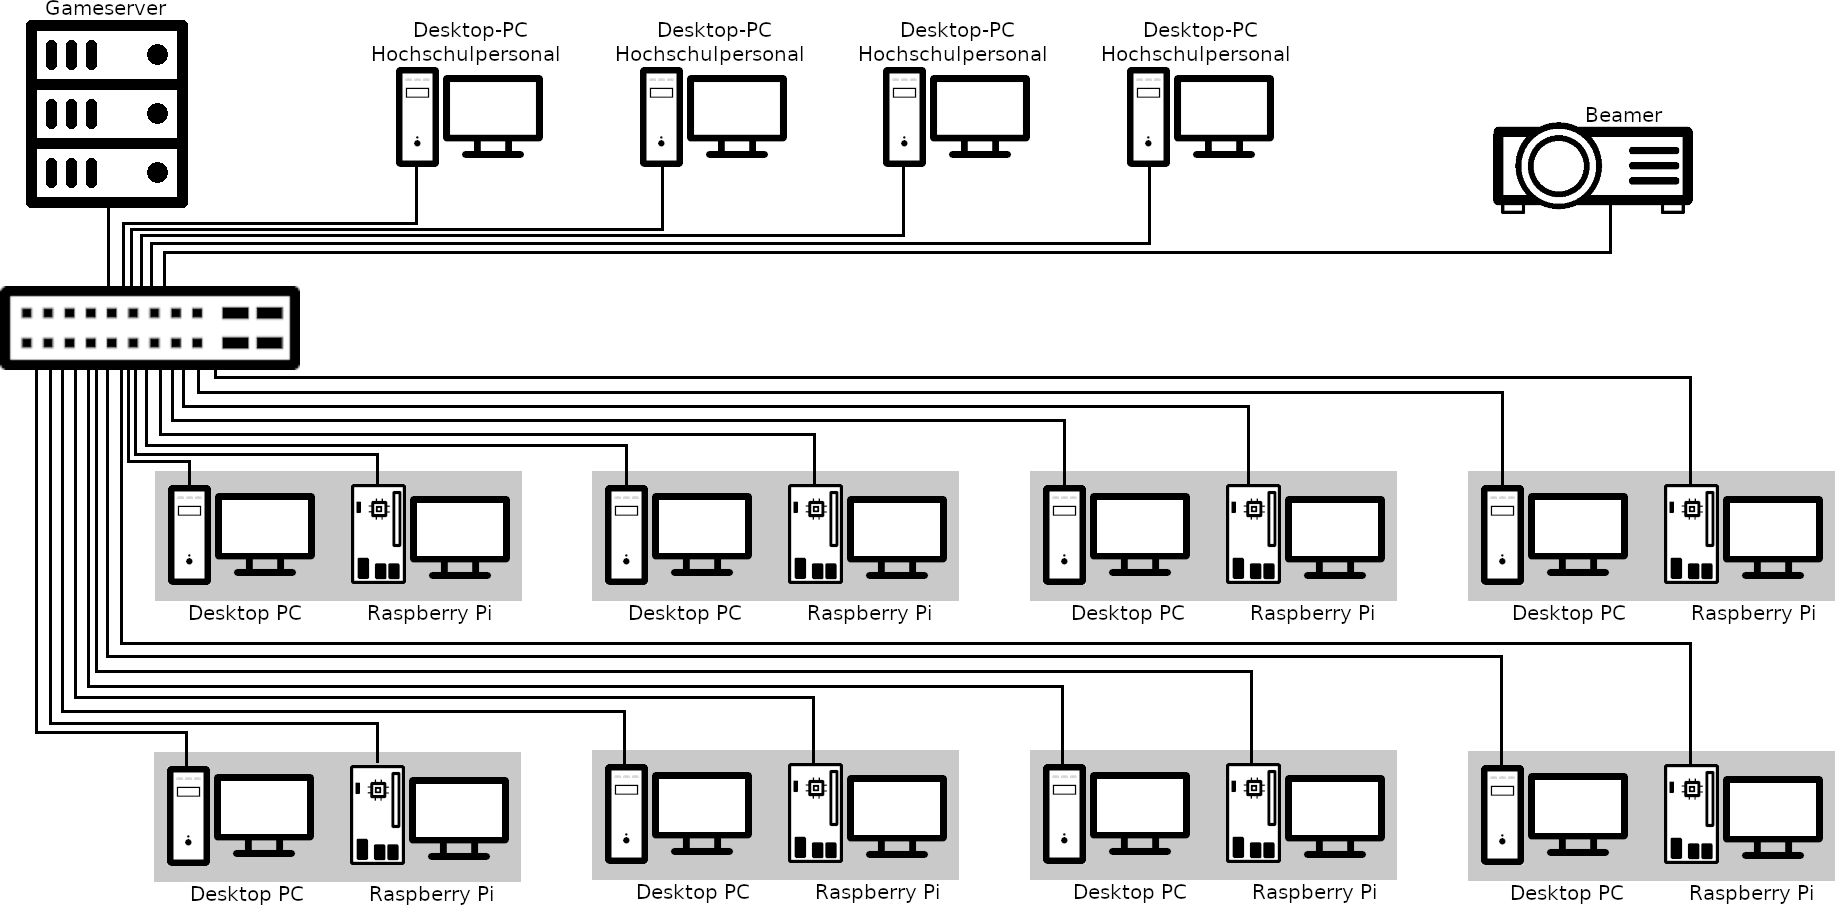
\includegraphics[width=\linewidth, keepaspectratio]{analyse/netzwerk-topologie-bak}
	\captionof{figure}{Übersicht über die Laborausstattung (Netzwerktopologie)}
	\label{fig:network-topology}
\end{center}

Wie in der \autoref{fig:network-topology} dargestellt, ist das Labor mit acht Gruppenarbeitsplätzen für Studierende sowie Arbeitsplätzen für die Mitarbeitenden ausgestattet. Ein Arbeitsplatz kann zu einem neunten Gruppenarbeitsplatz umfunktioniert werden.

An einem Gruppenarbeitsplatz (in der Abbildung \ref{fig:network-topology} grau hinterlegt) können 2 Studierende gleichzeitig arbeiten, da diese mit einem leistungsfähigen Desktop-PC und einem Raspberry Pi\footnote{Einplatinencomputer mit der Größe einer Kreditkarte} sowie den dazugehörigen Peripheriegeräten (Maus, Tastatur \& Monitor) ausgestattet sind.

Als Betriebssystem wird auf den Desktop-PCs Ubuntu\footnote{Ubuntu ist eine freie Linux Distribution auf Basis von Debian} und auf den Raspberry Pis Raspbian\footnote{Abwandlung von Debian für den Raspberry Pi} verwendet.

Auf den Desktop-PCs ist die Software VirtualBox der Firma Oracle installiert. Diese ermöglicht das Virtualisieren eines weiteren Rechners. Diese virtuelle Maschine wird Gast genannt und beheimatet die Dienste und Anwendungen, welche während des Versuchs benötigt werden. Durch die Nutzung der Virtualisierung muss die Software nicht auf dem Wirtsystem installiert werden. So ist dieses auch für andere Versuche im Rahmen der Lehrveranstaltung nutzbar, ohne dass auf Inkompatibilitäten von Softwares der verschiedenen Versuche geachtet werden muss. Auch bietet VirtualBox die Möglichkeit sogenannte Snapshots anzulegen. Ein Snapshot ist eine Momentaufnahme eines aktuellen Systemzustandes. Diese stellt eine Komplettsicherung des Systems dar und es ist möglich, die Systeme auf den gleichen Stand zu bringen. \cite{oraclecorporationOracleVMVirtualBox2020} Dies wird benötigt, um eine Vergleichbarkeit zwischen den Studierenden zu gewährleisten.

Die teilnehmenden Studentengruppen werden in den Softwarekomponenten und in der Auswertung durch die IP-Adresse ihres Gast-Systems identifiziert.

Neben diesen Rechner steht ein Linux Server zur Verfügung, auf welchem das Auswertungs- und Überwachungssystem betrieben wird.

Alle Rechner, auch die Gastsysteme der Studentengruppen, sind untereinander über ein Netzwerkswitch via Ethernet verbunden.

Außerdem steht ein Beamer zur Verfügung, auf dem die aktuelle Spielübersicht dargestellt werden kann.
	\section{Praktikum \textquote{Catch me, if you can}}
\label{sec:Praktikum}

Das zweite der drei Praktika \textquote{Catch me, if you can} wird im Rahmen eines Contest zwischen den teilnehmenden Studierenden Teams ausgetragen. Der Contest ist an ein CTF-Contest (Capture the Flag) angelehnt, nur dass die Teams Flags unter anderem auch durch das Hacken von anderen Teams erhalten können.

Der Contest ist in drei Phasen untergliedert.
\begin{enumerate}
	\item Vorbereitung
	\item Contest
	\item Abschluss
\end{enumerate}

\paragraph{Vorbereitung}\label{para:Vorbereitung}
Die Studierenden erhalten circa 30 Minuten Zeit, um ihr System in Betrieb zu nehmen und sich mit diesem vertraut zu machen. Auch ist es möglich das System – ohne dass dieses angegriffen werden kann – abzusichern.

\paragraph{Contest}\label{para:Contest}
Die Contestphase selber dauert circa 140 Minuten. In dieser Zeit dürfen die Studierenden sich untereinander Angreifen. Diese Zeit kann auch für die weitere Absicherung des eigenen Systems, die Lösung von zur Verfügung stehender Challenges sowie der Nutzung des Flagshops genutzt werden.

\paragraph{Abschluss}\label{para:Abschluss}
Nach Ende der Contestphase müssen die Studierenden ihre Angriffe einstellen und eine Flagabgabe ist nicht mehr möglich. Die Studierenden erstellen ein Screenshot der Punkteübersicht, um diesen in ihrem Bericht aufzunehmen. Eine Nachbesprechung ist optional und ist mit maximal 30 Minuten angesetzt.

Während des Contest gelten die folgenden Regeln:
\begin{itemize}
\item Der Gameserver darf nicht angegriffen werden!
\item Es dürfen nur die in Betrieb zu haltenden VirtualBox-Images angegriffen werden.
\item Denial of Service Angriffe sind nicht erlaubt.
\item Sollte eine Gruppe Root-Rechte auf einem angegriffen Rechner erlangen ist es verboten, Software auf
dem Rechner zu löschen oder durch Konfiguration unbrauchbar zu machen. Sie dürfen allein die Flags
auslesen.
\item Flags dürfen nicht modifiziert oder gelöscht werden!
\item Sämtliche Dienste müssen für den Gameserver (IP: 192.168.87.1) erreichbar bleiben!
\item Das Hauptverzeichnis des HTTP-Servers /var/www/ muss für alle Rechner erreichbar bleiben, andere
Verzeichnisse müssen für den internen Zugriff und extern über Username/Passwort zugänglich sein.
\item SSH- und der Datenbank-Server müssen für alle erreichbar sein
\item ftp-Server muss für alle erreichbar sein, Anonymous-Login ist nicht erforderlich.
\item ICMP-Pakete (ping) dürfen nicht blockiert werden!
\item  Das Passwort des Logins »gamemaster« darf nicht zurückgesetzt werden!
\end{itemize} \cite[S.9]{quadePraktikumITSecurity2017}\cite[S.10-11]{sosnaKonzeptionUndRealisierung2010}
	\section{Systemkomponenten}\label{sec:Systemkomponenten}

\subsection{Komponenten des Servers}\label{subsec:Komponente_des_Servers}
Im Folgenden werden die verschiedenen Komponenten des Auswertungs- und Überwachungssystems in der derzeitigen Implementierung untersucht. Dabei werden Rückschlüsse auf Anforderungen gezogen sowie Schwachstellen herausgearbeitet.

\subsubsection{Scanner}\label{subsubsec:Scanner}
Der Scanner prüft in regelmäßigen Abständen die auf den Gastsystemen der Studierenden installierten Dienste und speichert das Ergebnis ab. Die Abstände können beim Starten des Spieles eingestellt werden. Die folgenden Dienste werden pro Team geprüft.

\paragraph{ScanUp}\label{para:ScanUp}
Die Aufgabe dieses Scans besteht darin zu prüfen, ob das Gastsystem noch für den Server erreichbar ist. Sollte das Gastsystem nicht erreichbar sein, wird hierfür ein Strafpunkt vergeben. Aus technischer Sicht wird das Linux-Kommando \textit{ping} verwendet. Anhand des Rückgabewertes kann nachvollzogen werden, ob der Server das Gastsystem erreichen konnte.

\paragraph{ScanBubble}\label{para:ScanBubble}
Auf dem Gastsystem läuft ein selbst programmierter Bubble Server, welcher Flags unter Nutzung des Telnet Protokolls bereitstellt. Nachdem eine Flag abgeholt wurde, stellt der Dienst für eine bestimmte Zeit (Timeout) keine weiteren Flags bereit. Der Bubble Server nimmt Anfragen über den Port \textit{12321} für unverschlüsselte Flags und Port \textit{12322} für verschlüsselte Flags entgegen. Die Scan-Operation überprüft, ob eine Telnet-Verbindung zum Port \textit{12321} möglich ist, indem die Operation eine Telnet-Verbindung öffnet und prüft, ob die Verbindung erfolgreich war.
\newpage

\paragraph{ScanWebUp}\label{para:ScanWebUp}
Jedes Gastsystem stellt unter Zuhilfenahme eines Apache-Webservers und php-Dateien Webseiten und Daten bereit, die über einen Webclient abgerufen werden können. Dazu müssen auf Port \textit{80} der HTTP- und auf Port \textit{443} der HTTPS-Dienst laufen und erreichbar sein. Dieses verifiziert die Scan-Operation, indem sie eine Socket-Verbindung zu den Ports \textit{80} und \textit{443} öffnet und das Ergebnis prüft.

\paragraph{ScanSQLInjectUp}\label{para:ScanSQLInjectUp}
Dieser Scan prüft, ob die Login-Seite des Teams, auf der die SQL-Injection-Schwachstelle implementiert ist, erreichbar und benutzbar ist. Die Operation sendet hierzu eine valide Kombination aus Nutzername und Passwort an den Webserver. Das Ergebnis wird dann mit dem erwarteten Resultat verglichen.

\paragraph{ScanSQLInjectSave}\label{para:ScanSQLInjectSave}
Ähnlich wie bei der Operation ScanSQLInjectUp (\ref{para:ScanSQLInjectUp}) wird geprüft, ob Ergebnis und Erwartung übereinstimmen. Besonderheit hierbei ist, dass statt einer validen Kombination aus Nutzernamen und Passwort eine sogenannte SQL-Injection (wird im \autoref{subsec:Komponente_des_Clients} genauer erläutert) im Nutzernamen übergeben wird.  
Sollte die Anfrage alle gespeicherten Nutzerdaten zurückgeben, ohne dass eine Authentifizierung stattfindet, ist die SQL-Injection weiterhin möglich.

\paragraph{ScanXSSSave}\label{para:ScanXSSSave}
Diese Scan-Operation prüft, ob die auf dem Gastsystem implementierte XSS-Schwachstelle behoben wurde. Dazu wird die Webseite mit präpariertem Inhalt aufgerufen. Auf die Vorgehensweise wird im \autoref{subsec:Komponente_des_Clients} eingegangen.
In der Rückgabe wird geprüft, ob dieser ungefiltert auf der Webseite zu finden ist. Sollte dies der Fall sein, ist die XSS-Schwachstelle nicht oder unzureichend von den Studierenden abgesichert worden.

\paragraph{ScanSQLSave}\label{para:ScanSQLSave}
Bei diesem Scan wird kontrolliert, ob der Login mit dem auf allen Systemen voreingestellten Passwort \textit{toor} für den SQL-Account \textit{root} möglich ist. Ist dieser möglich, haben die Studierenden dieses unsichere Passwort nicht geändert. Des Weiteren wird geprüft, ob die Nutzerdaten in der htaccess-Datei, die die phpMyAdmin-Anwendung schützen soll, geändert worden sind.

\paragraph{ScanFTPSave}\label{para:ScanFTPSave}
Auf dem Client System läuft ein FTP-Server, der ohne Login (Nutzername \& Passwort) Daten bereitstellt. Der Scan prüft, ob ein sogenannter anonymer Login möglich ist, indem eine FTP-Verbindung ohne Login aufgebaut wird. Sollte die Verbindung erfolgreich sein, ist der anonyme Login immer noch nicht deaktiviert worden.

\paragraph{ScanTelnetSave}\label{para:ScanTelnetSave}
Ein Telnet-Server horcht auf Verbindungen auf Port \textit{23}. Da dieser Dienst nicht benötigt wird, soll er durch die Studierenden abgeschaltet oder deinstalliert werden. Die Scan-Operation prüft, ob eine Verbindung mithilfe des Telnet-Protokolls auf Port \textit{23} möglich ist. Dazu wird eine Verbindung zu Port \textit{23} aufgebaut und das Resultat geprüft.

\subsubsection{Generierung von Flags}\label{subsubsec:Generierung_von_Flags}

Derzeitig erfolgt die Generierung der Flags sowohl auf den Gastsystemen als auch auf dem Auswertungs- und Überwachungssystem. Dies ist notwendig, da ansonsten eine Überprüfung der Gültigkeit der Flags und Verrechnung der Punkte nicht durchgeführt werden kann. Die Flags werden durch einen Algorithmus generiert. Dieser erzeugt pro Team eine bestimmte Anzahl an Flags. 

Dazu wird die Flag mithilfe der Streuwertfunktion (Hashfunktion) MD5 und der Eingabe, einem sogenannten Seed, berechnet. Eine Hashfunktion bildet aus einer Eingabe variabler Länge eine Ausgabe mit einer festen Länge. Bei identischer Eingabe wird immer der gleiche Ausgabewert berechnet. Darüber hinaus ist es bei einer guten Hashfunktion nicht möglich, von der Ausgabe auf den Eingabewert zu schließen. \cite{menezesHandbookAppliedCryptography1996}

Der in der Anwendung genutzte Seed setzt sich aus der Verkettung von \textit{Salt}, \textit{IP-Adresse}, dem String \textquote{\textit{Aufgabe}} und einem \textit{Zähler} zusammen.

\begin{lstlisting}[, frame=single, caption={Beispiel eines Seed und seines Hashs}, captionpos=b, label={lst:analyse-hash-algo}]
seed = "WS2019192.168.87.11Aufgabe1"
hash = md5(seed)
hash = 7072D70B3D47E8516056A8B777655174
\end{lstlisting}

Ein Salt wird benötigt, um den Flags eine Lebenszeit zu geben. In der derzeitigen Implementierung enthält der Salt das aktuelle Jahr sowie das jeweilige Semester. So sind nur Flags des aktuellen Semesters gültig und werden vom Auswertungs- und Überwachungssystem akzeptiert. Einer Verwendung von Flags aus vorherigen Semestern wird somit effektiv vorgebeugt.

Die IP-Adresse stellt hierbei den Bezug zum jeweiligen Team dar.

Der String \textquote{Aufgabe} wird als Geheimnis verwendet, um das Fälschen von Flags zu erschweren und bestenfalls zu verhindern.

Damit pro Team mehrere eindeutige Flags generiert werden können, wird ein sogenannter Zähler genutzt. Dieser Zähler ist auf 0 initialisiert und wird pro generierter Flag um eins erhöht, bis die benötigte Anzahl an Flags generiert ist. \cite[S.48]{sosnaKonzeptionUndRealisierung2010}

\subsubsection{Webserver}\label{subsubsec:Webserver}

Der Webserver stellt das GUI (Graphical User Interface) für die Studierenden und betreuenden Personen dar. Hier kann der aktuelle Punktestand eingesehen werden. Auch wird in dem GUI dargestellt, welches Team welchen Service abgesichert hat, inklusive der Negativpunkte für nicht abgesicherte Dienste, und wie viele Strafpunkte das jeweilige Team erhalten hat.

Neben diesen Darstellungen befinden sich auf dem Server ein sogenannter Flagshop und diverse Challenges, mit denen Studierende weitere Flags erhalten können.

Die betreuenden Personen haben die Möglichkeit, über das Web-GUI ein neues Spiel anzulegen und das Spiel zu starten oder zu stoppen. Auch kann von dem Spiel ein Backup erstellt werden. Neben diesen Funktionen zur Spielsteuerung können an die Teams Strafen für unfaires oder regelverletzendes Verhalten verteilt werden. Diese nehmen direkten Einfluss auf die Punkte des jeweiligen Teams. Außerdem besteht die Möglichkeit, weitere Benutzer für das Administrationsinterface zu registrieren.

\paragraph{Flagshop} \label{para:Flagshop}
Der Flagshop ermöglicht es den Studierenden, weitere Flags mit ihren Punkten zu kaufen. Der Kauf von Flags lohnt sich, da die verkauften Flags mehr Punkte bringen als sie kosten. Um einen Einkauf im Flagshop durchzuführen, müssen die Teams vorher einen Account erstellen. Die Registrierung erfragt neben dem benötigten Benutzernamen und Passwort auch für den Flagshop irrelevante Daten ab. Diese ähneln persönlichen Informationen, die bei den meisten Onlineshops angegeben werden müssen. Das Format, hier die Repräsentation als Zahl oder String sowie die Länge, und die Erforderlichkeit der Daten werden nur im HTML-Formular festgelegt. Durch eine Manipulierung des Formulars kann dieses mit nicht konformen oder nicht vorhandenen Daten abgesendet werden. Für jede der nicht vorhandenen oder nicht konformen Informationen erhält der Studierende eine Flag. Daneben wird die \linebreak Güte des angegebenen Passwortes anhand von Länge und Anzahl an Sonderzeichen, Groß- und Kleinbuchstaben sowie Ziffern bewertet und mit Flags belohnt.

Nach der Registrierung können die Studierenden sich für ihre Punkte Flags kaufen. Dazu stehen zwei Pakete mit 8 bzw. 6 Flags für den Preis von jeweils 4 Punkten pro Paket zur Verfügung. Dieser Preis kann auf zwei Arten reduziert werden. 
Einmal müssen sich die beiden Pakete gleichzeitig im Warenkorb befinden und deren Identifikationsnummern (ID) müssen auf nicht vorhandene Nummern gesetzt werden. Die Manipulation resultiert in einem reduzierten Preis von 4 Punkten für beide Pakete. Dies ist extra im Flagshop einprogrammiert und soll die Studierenden auf Manipulation von IDs aufmerksam machen.
Durch die zweite Art ist es möglich, die Pakete kostenlos zu erhalten. Dazu muss im Warenkorb das sogenannte \textit{Hidden-Input-Feld}, in dem der aktuelle Preis des Warenkorbs gespeichert wird, auf 0 gesetzt werden. Dann berechnet der Flagshop für den Kauf einen Preis von 0 Punkten. \cite[S. 63]{abtsUeberarbeitungUndErweiterung2016}

Ein \textit{Hidden-Input-Feld} wird in der Repräsentation eines HTML-Dokumentes nicht angezeigt, kann jedoch durch die Entwicklertools eines Browser betrachtet und verändert werden. \cite{w3schoolsHTMLHiddenInput}

Auf diese Weise ist es auch möglich, einen negativen Preis festzulegen und dem eigenen Team Punkte zuzuschreiben, da die derzeitige Implementierung nicht prüft, ob der von dem Nutzenden eingegebene Preis kleiner als 0 ist, sondern ob dieser gleich 0 ist. Bei korrekter Implementierung würde ein Preis kleiner 0 geprüft und korrigiert.

\paragraph{Challenges} \label{para:Challenges}
Derzeitig sind fünf Challenges implementiert, die vom System in zufälliger Reihenfolge an interessierte Teams verteilt werden. Eine abgeschlossene oder abgebrochene Challenge, durch das Neuladen der Webseite oder durch das Betätigen der Zurück-Taste, kann nicht wiederholt werden. Eine Challenge kostet 10 Punkte. Nach erfolgreichem Abschluss einer Challenge gibt es 10 Punkte plus eine gewisse Anzahl an Punkten für das Absolvieren der Aufgabe. Die folgenden Challenges sind implementiert: \cite[S.19]{abtsUeberarbeitungUndErweiterung2016}

\subparagraph{Aufgabe 1: robots.txt}\label{subpara:Aufgabe_1_robots.txt}
Die Studierenden sollen in dieser Challenge lernen, dass die \textit{robots.txt} Datei keinen Zugriffsschutz darstellt. Diese bittet nur Suchmaschinen, die angegebenen Verzeichnisse und Dateien nicht zu indexieren. Aus der \textit{robots.txt} Datei können Informationen zu versteckten Dateien und Verzeichnissen erhalten werden. Die Studierenden sollen über die \textit{robots.txt} Datei einen vorhandenen Ordner finden. In diesem befindet sich die Lösung zur Challenge. \cite[S.19-20]{abtsUeberarbeitungUndErweiterung2016}

\subparagraph{Aufgabe 2: JavaScript-Login-Bypass}\label{subpara:Aufgabe_2_JavaScript-Login-Bypass}
Bei dieser Challenge ist das benötigte Passwort zur Lösung der Challenge als Klartext im Quelltext versteckt. Das Verstecken wird derzeitig mit einer Meldung wie \textquote[\cite{abtsUeberarbeitungUndErweiterung2016}]{Seitenquelltext deaktiviert} und vielen Leerzeilen realisiert. Im Inspector von Firefox Version 78.0.1 und Chromium Version 83.0.4103.116 ist dies nicht möglich, da die Leerzeilen entfernt werden und das Passwort daher oben im Quelltext zu sehen ist. \cite[S.20]{abtsUeberarbeitungUndErweiterung2016}

\subparagraph{Aufgabe 3: Form-Modification}\label{subpara:Aufgabe_3_Form-Modification}
In dieser Challenge sollen die Studierenden verstehen, dass auch die Werte von Drop-Down-Menüs, Checkboxen und Radio-Buttons durch Manipulation auf nicht vorgegebene Werte geändert werden können. Deshalb müssen Nutzereingaben stets auch serverseitig überprüft werden, da hier die Regeln der Überprüfung nicht durch den Nutzenden verändert werden können.

Die Aufgabe besteht darin, einen bestimmten Login-Namen aus einem Drop-Down-Menü auszuwählen. Da der geforderte Name nicht in dieser Liste ist, müssen die Studierenden das HTML-Formular so manipulieren, dass er auswählbar ist. \cite[S.20]{abtsUeberarbeitungUndErweiterung2016}

\subparagraph{Aufgabe 4: JavaScript-Substrings}\label{subpara:Aufgabe_4_JavaScript-Substrings}
Das Passwort, das die Studierenden eingeben müssen, wird clientseitig mithilfe einer JavaScript Funktion geprüft. Damit das Passwort nicht im Klartext im Quelltext steht, wird dieses verschleiert. So werden drei Strings Zeichen für Zeichen verglichen. Sollte ein Zeichen in mindestens zwei der drei Strings übereinstimmen, dann gehört dieses Zeichen zum Passwort. Im Anschluss wird geprüft, ob das generierte Passwort gleich dem ist, das die Studierenden als Passwort genutzt haben. \cite[S.20]{abtsUeberarbeitungUndErweiterung2016}

\subparagraph{Aufgabe 5: URL-Hex-Injection}\label{subpara:Aufgabe_5_URL-Hex-Injection}
Die Studierenden sollen an geheime Informationen in einem Ordner gelangen, der nach einem Wert aus dem Hexadezimalsystem benannt ist. Anders als im Dezimalsystem ist die Basis 16 statt 10. Die Aufgabe soll zeigen, dass Ordner, die nach einem Hexadezimalwert benannten sind, auf diese Art und Weise nicht vor Zugriffen geschützt werden können, da das Präfix Zeichen \textit{\%} für Hexadezimalzahlen selbst durch einen Hexadezimalwert (\%25) dargestellt werden kann. \cite[S.20]{abtsUeberarbeitungUndErweiterung2016}

\subsubsection{Abgabe von Flags}\label{subsubsec:Abgabe_von_Flags}
Um Flags abgeben zu können, müssen die Studierenden sich mit ihren Zugangsdaten, die sie durch das Lösen des Hackits erhalten haben, in der Web-GUI anmelden. Dort ist es möglich, in einem Input-Feld eine Flag synchron abzugeben. Das bedeutet, dass nach jeder Abgabe die Webseite neu geladen wird. Eine Abgabe mehrere Flags ist gleichzeitig nicht möglich.

\subsection{Komponenten des Clients}\label{subsec:Komponente_des_Clients}
Da sich die Bachelorarbeit mit der Modernisierung des Auswertungs- und Überwachungssystems beschäftigt, sind nur die für die Bachelorarbeit wichtigen Komponenten des Clients beschrieben.

\subsubsection{Webserver des Clients}\label{subsubsec:Webserver_des_Clients}
Auf den Clients wird ein Webserver mit einigen extra implementierten Schwachstellen betrieben. Diese sollen während des Versuches durch die Studierenden behoben werden.

Der Webserver stellt eine Art Kundenbewertungsformular mit implementierter XSS Schwachstelle bereit. In der verwendeten Implementierung wird die Eingabe des Nutzers in das HTML-Dokument geschrieben. Durch die Schwachstelle wird eine Nutzereingabe ungefiltert in das HTML-Formular übernommen und ein potenziell schädlicher Code wird vom Browser verarbeitet. Dieser Code kann dann beispielsweise vertrauliche Informationen wie Cookies, Session-Tokens oder persönliche Daten auslesen und den Angreifern übermitteln. \cite{ruettenSicherheitWebanwendungen2007}

Eine weitere Schwachstelle stellt der sogenannte \textquote{Login zum Membersbereich} mit der implementierten SQL-Injection Schwachstelle dar. 
Bei einer SQL-Injection versucht ein Angreifer den verwendeten SQL-Befehl so zu erweitern, dass dieser neben der eigentlichen Abfrage an die Datenbank auch einen vom Angreifer vorbereiteten SQL-Befehl ausführt. Die Erweiterung des SQL-Befehls erfolgt, indem die Eingabe, die in den SQL-Befehl aufgenommen wird, das Zeichen für das Ende des SQL-Befehls inklusive des vom Angreifer intendierten SQL-Befehls enthält. Über diesen Angriff können dann unerlaubterweise Daten ausgelesen werden, aber auch eine Löschung der Daten ist denkbar. \cite{bachfeldGiftspritze2004}

In der verwendeten Implementierung werden der Benutzername und das Passwort ungefiltert in den SQL-Befehl übernommen. Diese Schwachstelle lässt sich erst beheben, wenn die Gruppe die SQL-Injection bei sich selbst erfolgreich durchgeführt hat. \cite[S.27-29]{abtsUeberarbeitungUndErweiterung2016}

Neben diesen Schwachstellen gibt es eine Registrierung für den Flagshop. Diese erfordert einige Eingaben wie Name, Alter, Postleitzahl und vieles mehr. Die Eingaben sind im HTML-Formular als Pflicht markiert und haben eine Vorgabe in der Form. Ein Absenden ist ohne Angabe dieser Daten nicht möglich. Die Studierenden erhalten jedoch für jede nicht getätigte und für jede nicht der Form entsprechenden Angabe Flags nach der Registrierung. \cite[S.26]{abtsUeberarbeitungUndErweiterung2016} Dies ist möglich, da das HTML-Formular durch die Studierenden geändert werden kann und der Server nur die Angaben bezüglich Passwort und Nutzername prüft. Diese beiden Angaben werden genutzt, um sich am Flagshop des Servers anzumelden und Flags zu erwerben. \textit{(Siehe: \autoref{para:Flagshop} Flagshop)}

Außerdem stellt der Webserver eine Bildergalerie zur Verfügung. In dieser befinden sich zum Spielstart zwei normal erscheinende Bilder. Entgegen dem Anschein sind in diesen Flags verschleiert. Die Steganografie wird durch die Kombination eines Bildes und eines ZIP-Archivs erreicht. \cite[S.27]{abtsUeberarbeitungUndErweiterung2016}
	\section{Schnittpunkte zwischen Server und Clients}
\label{sec:Schnittpunkte_zwischen_Server_und_Clients}

Der Server und die Clients laufen auf getrennten Systemen. Da die Studierende Schwachstellen auf ihren Clients beheben sollen, muss das Auswertungs- und Überwachungssystem auf diese Systeme zugreifen. Dadurch lassen sich die folgenden Schnittpunkte begründen.

Die Scanner prüfen vom Auswertungs- und Überwachungssystem aus, ob 
\begin{itemize}
	\item das System online ist,
	\item der Webserver erreichbar ist,
	\item der Bubble-Server erreichbar ist,
	\item der Login zum Membersbereich erreichbar und abgesichert ist,
	\item die Kundenbewertung erreichbar und abgesichert ist,
	\item ob das SQL Passwort geändert worden ist,
	\item ob der FTP Server gegen unautorisierten Zugriff abgesichert ist und
	\item ob der Telnet Dienst auf Port 23 abgeschaltet ist. 
\end{itemize}

Des Weiteren verbinden sich die Clients beim Starten mit dem Auswertungs- und Überwachungssystem um Flags für die Flagshop-Registrierung und -Anmeldung zur Verfügung zu stellen.
	\section{Abgeleitete Anforderungen}
\label{sec:Abgeleitete_Anforderungen}

Das Auswertungs- und Überwachungssystem muss anhand der vorhergehenden Analyse folgenden Anforderungen genügen:
\begin{itemize}
	\item Überwachung von mindestens neun Studierendensystemen
	\item Ermittlung und Sicherung der Zustände von Diensten, welche auf den Studierendensystemen angeboten werden müssen
	\item Entgegennahme und Prüfung von Flags, inkl. der Verrechnung von (Straf-)Punkten
	\item Ermittlung und Visualisierung der Teilergebnisse sowie des Gesamtergebnisses
	\item Informationsvermittlung aller Dienst- und Punkteänderungen durch unter anderem \\ Dienststatusänderung, Flagabgabe und Strafen (fortlaufende Publikation für Studierende und betreuende Personen)
	\item Dokumentation aller Events durch Protokollierung der einzelnen Aktionen des Systems
	\item Bereitstellung von Challenges, damit Studierende sich weitere Punkte erarbeiten können
	\item Bereitstellung eines (Flag-) Shops, bei dem mehrere Sicherheitslücken ausgenutzt werden können, um Flags zu erhalten
	\item Einstellungen des Spiels sollen durch betreuende Personen geändert werden können
	\item Verwaltung von Benutzern (administrierende, betreuende und spielende Personen)
	\item Zugangskontrolle für teilnehmende Studierende durch Prüfung der Hackits
	\item Sicherung alter Spielstände.
\end{itemize}
	
	\chapter{Entwurf}
	\label{chap:Entwurf}
	%\input{40-Entwurf/xyz}
	
	\chapter{Technologien}
	\label{chap:Technologien}
	%\input{50-Entwurf/xyz}
	
	\chapter{Realisierung}
	\label{chap:Realisierung}
	%\input{60-Realisierung/xyz}
	
	\chapter{Ergebnis}
	%\input{60-Ergebnis/xyz}
	
	\chapter{Zusammenfassung \& Aussicht}
	%\input{70-Ende/xyz}
	
	% Nachspann einleiten:
	\backmatter 
	% Einstellungen für die Fußzeile aktualisieren
	% 	Einstellungen nur für die rechten Seiten
	% 	Layout: Abschnitt  |  Seite
	\rofoot[\textbf{$\mid$~~\pagemark}]{\textbf{$\mid$~~\pagemark}}
	%	Einstellungen nur für die linken Seiten
	%	Layout: Seite  |  Kapitel
	\lefoot[\textbf{\pagemark~~$\mid$}]{\textbf{\pagemark~~$\mid$}}
	\chapter{Anhang}
	%\input{90-Anhang/xyz}
	
	% Tabellenverzeichnis
	\listoffigures
	
	% Abbildungsverzeichnis
	\listoftables
	
	% Codeverzeichnis
	\lstlistoflistings
	
	% Quellenverzeichnis
	\printbibliography
	 
	% Stichwortverzeichnis
	\printindex
	
\end{document}